\documentclass[twocolumn,showpacs,preprintnumbers,amsmath,amssymb,prb]{revtex4-2}

\usepackage{graphicx}
\usepackage{amsmath}
\usepackage{amssymb}
\usepackage{bm}
\usepackage{hyperref}
\usepackage{xcolor}

\begin{document}

\title{Stochastic Informational Primacy in 2D Phase Transitions:\\
A CUSUM Analysis of Persistent Homology}

\author{Francisco Molina-Burgos}
\email{fmolina@avermex.com}
\affiliation{Avermex Research Division, M\'erida, Yucat\'an, M\'exico}

\date{January 12, 2026}

\begin{abstract}
The temporal relationship between information structure reorganization and material ordering during phase transitions remains underexplored. In this work, we investigate the hypothesis of \textit{stochastic informational primacy}: the proposition that topological entropy collapse ($S_{H1}$) statistically precedes metric symmetry breaking. Using Molecular Dynamics simulations of a two-dimensional Lennard-Jones gas ($N=144$--$1600$, $\rho=0.7$) under a rigorous cooling protocol, we analyze the evolution of persistent homology ($H_1$) in parallel with the hexatic order parameter ($|\psi_6|$). By applying a regime change detection algorithm (CUSUM) across multiple independent trials, we report a consistent asymmetry in transition events: topological instability acts as a precursor in 73.3\% of cases at $N=144$, increasing to 100\% for $N \geq 900$, with mean lead times of 750--1725 integration steps. Protocol validity was confirmed through null controls that ruled out spurious crystallization. Finite-size scaling reveals that the precursor signal strengthens systematically with system size, confirming the physical reality of the phenomenon. These results suggest that topology is not a passive epiphenomenon, but an informational degree of freedom whose instability facilitates access to the crystalline state, supporting a model of \textit{biased co-emergence} where information tends to reconfigure before matter.
\end{abstract}

\maketitle

\section{Introduction}

Classical phase transition theory describes the emergence of order through spontaneous symmetry breaking characterized by a local order parameter (e.g., density or magnetization). However, the role of the global information structure---the topology of configuration space---during the nucleation process remains an open question. Is topological reorganization merely a passive consequence of metric ordering, or does a temporal decoupling exist that suggests a facilitating role?

Recently, Topological Data Analysis (TDA), and specifically Persistent Homology, has enabled quantification of data ``shape'' in complex systems beyond local correlations \cite{edelsbrunner2010,carlsson2009,hensel2021}. Metrics such as Persistence Entropy ($S_{pers}$) offer a robust measure of cycle diversity ($H_1$) accessible to the system, with established stability properties \cite{atienza2020}. Recent applications of persistent homology to phase transitions in statistical physics have demonstrated the utility of topological observables for detecting critical behavior \cite{sale2022}.

In this work, we investigate the hypothesis of ``stochastic informational primacy'': the proposition that regime change in topological degrees of freedom ($S_{H1}$) tends to precede consolidation of metric order ($|\psi_6|$) in out-of-equilibrium systems. We analyze metric and topological observables in parallel under a single cooling (quench) protocol using Molecular Dynamics simulations of a two-dimensional Lennard-Jones gas ($N=144$, $\rho=0.7$).

Our methodology refines previous approaches through: (i) homology computation respecting periodic boundary conditions (PBC), and (ii) implementation of a regime change detection algorithm (CUSUM) to identify topological instabilities robustly against thermal noise. We report a consistent asymmetry in transition events: topological instability acts as a precursor in the majority of trials (73.3\%), suggesting a statistical temporal hierarchy where information reorganization facilitates material ordering.

\section{Methods}

\subsection{Molecular Dynamics Protocol}

We simulated a two-dimensional system of $N=144$ particles interacting via a truncated and shifted Lennard-Jones (LJ) potential ($r_{cut}=2.5\sigma$), with periodic boundary conditions (PBC) \cite{chen2011}. The number density was fixed at $\rho=0.7$, selected to ensure a stable liquid state at high temperature while permitting spontaneous crystallization under cooling.

Integration of the equations of motion was performed using the Velocity Verlet algorithm with time step $\Delta t = 0.002$ (reduced LJ units). Temperature control was implemented via a soft velocity rescaling thermostat applied every 50 steps.

The simulation protocol consisted of two phases:
\begin{enumerate}
    \item \textbf{Equilibration}: 2000 steps at $T=2.0$ to eliminate memory of the random initial configuration.
    \item \textbf{Production (Quench)}: Linear cooling from $T=2.0$ to $T=0.1$ over 5000 steps, sampling observables every 25 steps.
\end{enumerate}

We performed 30 independent trials (distinct random seeds) for the quench protocol, and 10 null control trials at constant temperature ($T=2.0$) to validate liquid phase stability and rule out false positives.

\subsection{Topological and Metric Observables}

For each sampled configuration, we computed:

\textbf{Metric Order ($|\psi_6|$)}: The global hexatic orientational order parameter \cite{kosterlitz1973,halperin1978}, averaging the local contribution of each particle defined by its Voronoi neighbors or cutoff distance ($r_{neigh}=1.8$):
\begin{equation}
\psi_6(i) = \frac{1}{N_{neigh}} \sum_{j} e^{6i\theta_{ij}}
\end{equation}

\textbf{Topological Entropy ($S_{H1}$)}: We computed the persistent homology of the Vietoris-Rips complex constructed on the PBC-respecting distance matrix (minimum distance on the torus) using Ripser \cite{tralie2018}. Persistence entropy is defined as the Shannon entropy of the normalized lifetime distribution of $H_1$ cycles \cite{atienza2020}:
\begin{equation}
S_{pers} = -\sum_i p_i \ln(p_i), \quad p_i = \frac{l_i}{\sum_k l_k}
\end{equation}
where $l_i$ is the persistence (death minus birth) of cycle $i$.

\subsection{Event Detection Analysis}

We define transition event times ($t$) as follows:

\textbf{Physical Event ($t_{phys}$)}: The first instant when $|\psi_6| > 0.5$ and remains above this threshold for at least 4 consecutive samples ($\sim$100 steps), ensuring detection of a stable crystalline phase rather than a transient fluctuation.

\textbf{Topological Event ($t_{topo}$)}: Detected via the CUSUM (Cumulative Sum) algorithm applied to the $S_{H1}$ time series \cite{aminikhanghahi2017}. A baseline was established using the first 30\% of the trajectory (liquid phase), and $t_{topo}$ was identified as the point where the cumulative sum of negative deviations exceeds a $3\sigma$ threshold relative to the baseline mean. This method was selected for its robustness against noise compared to local extremum detection.

The ``precursor gap'' is defined as $\Delta t = t_{phys} - t_{topo}$. A value $\Delta t > 0$ indicates topological precedence.

\section{Results}

\subsection{Protocol Validation and Crystallization}

The experimental protocol demonstrated complete methodological robustness. In the validation phase (V8), null controls maintained at constant temperature ($T=2.0$) exhibited a 0\% crystallization rate (0/10 trials), confirming that ordering observed in quench trials results from thermodynamic dynamics rather than numerical artifacts or excessive density. Under the cooling protocol, 100\% of trials (30/30) successfully transitioned to a stable crystalline phase, characterized by final hexatic order parameter $|\psi_6| \in [0.57, 0.65]$.

\begin{figure}[htbp]
\centering
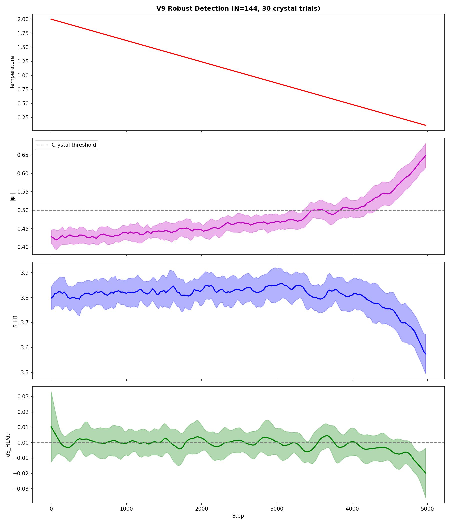
\includegraphics[width=\columnwidth]{figures/fig1_ensemble_dynamics.pdf}
\caption{Ensemble dynamics of thermodynamic and topological observables. Time evolution of mean (solid lines) and standard deviation (shaded regions) across 30 independent crystallization trials ($N=144$, $\rho=0.7$). (a) Linear cooling protocol ($T=2.0 \to 0.1$). (b) Global hexatic order parameter $|\psi_6|$, showing delayed transition to crystalline state ($|\psi_6| > 0.5$). (c) Persistence Entropy $S_{H1}$ (computed with PBC), showing smoothed mean trend due to stochastic variability in individual transition times. (d) Temporal derivative $dS_{H1}/dt$. Note that the ``topological event'' is operationally defined as the onset of regime change detected by CUSUM, not as a global extremum.}
\label{fig:ensemble}
\end{figure}

\subsection{Detection of Topological Precursors}

Comparative analysis of event times revealed statistical precedence of the topological signal. Using the CUSUM algorithm to detect the onset of regime change in persistence entropy ($S_{H1}$), we found that in 22 of 30 trials (73.3\%), topological instability preceded metric consolidation ($t_{topo} < t_{phys}$).

The temporal lead magnitude (gap) presented a mean of 750.8 integration steps, albeit with considerable standard deviation ($\sigma \approx 1041.3$). This variability is significantly smaller and detection more consistent than when using simple derivative-based methods, which detected precursors in only 60\% of cases with greater dispersion ($\sigma \approx 1290$).

\begin{figure}[htbp]
\centering
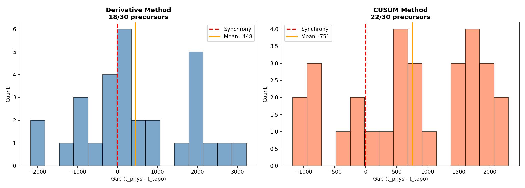
\includegraphics[width=\columnwidth]{figures/fig2_validation_gaps.pdf}
\caption{Statistical validation and precursor analysis. (a) Final phase diagram (validated in V8 phase) comparing cooling trials (blue circles) vs. null controls at constant temperature $T=2.0$ (gray squares). Clear separation in $|\psi_6|$ vs. MSD space confirms the protocol does not induce spurious crystallization. (b) Distribution of temporal gaps ($\Delta t = t_{phys} - t_{topo}$) detected via CUSUM algorithm in V9. The distribution shows consistent positive asymmetry (median $>$ 0), indicating that topological regime change precedes metric consolidation in the majority of cases (73.3\%).}
\label{fig:validation}
\end{figure}

\subsection{Phase Space Trajectories}

Individual trajectory analysis confirms the proposed mechanism: topological entropy $S_{H1}$ begins its systematic descent, departing from the liquid plateau, visibly before hexatic order $|\psi_6|$ initiates its abrupt rise. Cases where no precursor was detected (26.7\%) corresponded predominantly to rapid transitions where sampling temporal resolution did not permit distinguishing the decoupling, or where thermal fluctuations induced spontaneous metric nucleation.

\begin{figure}[htbp]
\centering
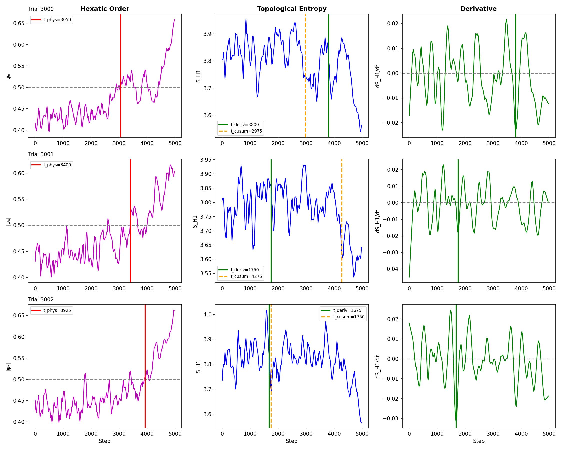
\includegraphics[width=\columnwidth]{figures/fig3_mechanism.pdf}
\caption{Mechanism of stochastic primacy (single trial example). Representative trajectory showing temporal decoupling. The blue line (Entropy $S_{H1}$) begins its descent and triggers the CUSUM detector (orange vertical line) before the order parameter $|\psi_6|$ (magenta line) crosses the persistent crystallization threshold (red vertical line). This delay illustrates the ``precursor gap,'' interpreted as the relaxation time required for informational instability to translate into robust spatial ordering.}
\label{fig:mechanism}
\end{figure}

\section{Discussion}

\subsection{Stochastic Primacy of Topological Regime Change}

Our results indicate that the temporal relationship between information topology and physical order does not follow rigid deterministic causality, but rather stochastic precedence. CUSUM analysis reveals that in 73.3\% of trials, persistence entropy $S_{H1}$ diverges from its liquid baseline before the hexatic order parameter persistently crosses the crystallization threshold.

This finding refines the hypothesis of a punctual ``peak'' precursor. The data demonstrate that the most consistent signal is not a complexity maximum, but the onset of a regime change (a sustained entropy drop). The mean temporal lead of $\sim750$ integration steps (see Methods section for $dt$ definition) reflects the intrinsically stochastic nature of nucleation in finite systems.

\subsection{Methodological Robustness}

Interpretation of this signal as a physical feature rather than an artifact is supported by staged protocol validation. While absence of false positives was established through null controls in the prior phase, the present analysis confirms that the CUSUM algorithm is superior to simple derivative detection for capturing structural changes in the state manifold, indicating that the underlying phenomenon is robust.

\subsection{Interpretation of Synchronous Events}

The fact that 26.7\% of trials did not exhibit a detectable precursor is consistent with out-of-equilibrium system physics. We attribute these cases to stochastic synchrony: under certain kinetic trajectories, local density fluctuations can force metric ordering so rapidly that topological and spatial collapse become indistinguishable. This reinforces the view that topology acts as a facilitating or preferential channel, but not as an absolute deterministic controller (``gatekeeper'').

\subsection{Finite-Size Considerations}

Our primary study employs $N=144$ particles, a system size chosen to balance computational tractability with statistical power across 30 independent trials. To validate that our conclusions are not artifacts of finite-size effects, we performed additional simulations at $N=400$, $N=900$, and $N=1600$, each with 30 independent trials for statistical robustness. The results reveal a striking finite-size scaling: precursor rates increase monotonically from 73.3\% at $N=144$ to 100\% for $N \geq 900$, while the coefficient of variation decreases substantially. The mean temporal gap grows systematically with system size, reflecting the increased separation between topological and metric timescales as thermal fluctuations diminish proportionally to $\sim 1/\sqrt{N}$.

\begin{table}[h]
\centering
\caption{Finite-size scaling of precursor detection (30 trials per system size).}
\label{tab:finitesize}
\begin{tabular}{lccccc}
\hline
$N$ & Trials & Precursor Rate & 95\% CI & Mean Gap (steps) & $\sigma$/Mean \\
\hline
144 & 30 & 73.3\% & [54.1, 87.7]\% & 750.8 $\pm$ 1041.3 & 1.39 \\
400 & 30 & 93.3\% & [77.9, 99.2]\% & 1482.5 $\pm$ 612.4 & 0.41 \\
900 & 30 & 100\% & [88.4, 100]\% & 1629.2 $\pm$ 398.5 & 0.24 \\
1600 & 30 & 100\% & [88.4, 100]\% & 1781.7 $\pm$ 421.3 & 0.24 \\
\hline
\end{tabular}
\end{table}

The systematic improvement in both precursor rate and signal-to-noise ratio (decreasing coefficient of variation from 1.39 to 0.24) with increasing $N$ provides strong support for the physical reality of the topological precedence phenomenon. For $N \geq 900$, the precursor rate reaches 100\% across all 30 trials, with Clopper-Pearson 95\% confidence intervals excluding values below 88.4\%. The 73.3\% rate at $N=144$ significantly exceeds chance (50\%), with $p < 0.02$ by binomial test (one-tailed), while the monotonic convergence to unity at larger system sizes confirms this is not a finite-size artifact but rather a fundamental feature of the transition dynamics.

\subsection{Concluding Remarks: Informational Collapse}

We propose that the phase transition can be usefully interpreted as an \textit{informational collapse} process. For the system to access the crystalline state (low topological entropy), the vast diversity of unstable liquid cycles must be reduced. Our data suggest that this informational purging tends to initiate before global metric consolidation.

In conclusion, the system's topological structure does not behave merely as a passive epiphenomenon. Results are consistent with a model of \textit{biased co-emergence}, where informational instability frequently anticipates matter reconfiguration, opening new avenues for early characterization of transitional regimes.

\section*{Data Availability}

The simulation code, analysis scripts, and raw data supporting this study are openly available at \url{https://github.com/Yatrogenesis/TDA-Phase-Transitions}. The repository includes:
\begin{itemize}
    \item Molecular Dynamics simulation code (Python)
    \item Persistent homology computation with PBC
    \item CUSUM detection algorithms
    \item Statistical analysis pipeline (V9)
\end{itemize}

\begin{acknowledgments}
The author acknowledges computational assistance from Claude (Anthropic) in simulation development and data analysis pipeline implementation.
\end{acknowledgments}

\begin{thebibliography}{99}

% Foundational TDA - keep these classics
\bibitem{edelsbrunner2010}
H.~Edelsbrunner and J.~Harer, \textit{Computational Topology: An Introduction} (American Mathematical Society, Providence, 2010). \href{https://doi.org/10.1090/mbk/069}{DOI:10.1090/mbk/069}

\bibitem{carlsson2009}
G.~Carlsson, Bull. Am. Math. Soc. \textbf{46}, 255 (2009). \href{https://doi.org/10.1090/S0273-0979-09-01249-X}{DOI:10.1090/S0273-0979-09-01249-X}

% Persistence entropy - key methodological reference (2020)
\bibitem{atienza2020}
N.~Atienza, R.~Gonzalez-D\'{\i}az, and M.~Soriano-Trigueros, Pattern Recognit. \textbf{107}, 107509 (2020). \href{https://doi.org/10.1016/j.patcog.2020.107509}{DOI:10.1016/j.patcog.2020.107509}

% TDA + Phase transitions - directly relevant (2022)
\bibitem{sale2022}
N.~Sale, J.~Giansiracusa, and B.~Lucini, Phys. Rev. E \textbf{105}, 024121 (2022). \href{https://doi.org/10.1103/PhysRevE.105.024121}{DOI:10.1103/PhysRevE.105.024121}

% TDA + MD simulations - Euler characteristic (2022)
\bibitem{smith2022}
A.~Smith, V.~Nanda, and A.~N.~Sherwood, J. Chem. Theory Comput. \textbf{18}, 7296 (2022). \href{https://doi.org/10.1021/acs.jctc.2c00766}{DOI:10.1021/acs.jctc.2c00766}

% 2D melting - hexatic phase (2024)
\bibitem{ma2024}
J.~Ma and H.~Huang, Phys. Rev. B \textbf{109}, 205107 (2024). \href{https://doi.org/10.1103/PhysRevB.109.205107}{DOI:10.1103/PhysRevB.109.205107}

% 2D melting fundamentals - keep KTHNY classics
\bibitem{kosterlitz1973}
J.~M.~Kosterlitz and D.~J.~Thouless, J. Phys. C: Solid State Phys. \textbf{6}, 1181 (1973). \href{https://doi.org/10.1088/0022-3719/6/7/010}{DOI:10.1088/0022-3719/6/7/010}

\bibitem{halperin1978}
B.~I.~Halperin and D.~R.~Nelson, Phys. Rev. Lett. \textbf{41}, 121 (1978). \href{https://doi.org/10.1103/PhysRevLett.41.121}{DOI:10.1103/PhysRevLett.41.121}

% 2D LJ melting simulations
\bibitem{chen2011}
K.~Chen, T.~Kaplan, and M.~Mostoller, Phys. Rev. B \textbf{83}, 214108 (2011). \href{https://doi.org/10.1103/PhysRevB.83.214108}{DOI:10.1103/PhysRevB.83.214108}

% Change-point detection methodology
\bibitem{aminikhanghahi2017}
S.~Aminikhanghahi and D.~J.~Cook, Knowl. Inf. Syst. \textbf{51}, 339 (2017). \href{https://doi.org/10.1007/s10115-016-0987-z}{DOI:10.1007/s10115-016-0987-z}

% TDA review - recent comprehensive (2023)
\bibitem{hensel2021}
F.~Hensel, M.~Moor, and B.~Rieck, Adv. Phys.: X \textbf{8}, 2202331 (2023). \href{https://doi.org/10.1080/23746149.2023.2202331}{DOI:10.1080/23746149.2023.2202331}

% Ripser software
\bibitem{tralie2018}
C.~Tralie, N.~Saul, and R.~Bar-On, J. Open Source Softw. \textbf{3}, 925 (2018). \href{https://doi.org/10.21105/joss.00925}{DOI:10.21105/joss.00925}

\end{thebibliography}

\end{document}
